
%\chapter{Method}
\chapter{Tools and methodology}
This section describes the process of planning and implementing an emulator for the Game Boy, the tools used and why they were chosen.% and is followed by the results, presenting what was achieved.
%\section{Tools and methodology}
\section{Programming language}
The language used in the project is C++ \cite{c++}. The language was chosen because it is fast, and supports the bit-level manipulation that is required when emulating hardware.
\section{Graphics and GUI}
For displaying graphics SDL2 \cite{SDL2} and OpenGL \cite{OpenGL} were chosen, mainly due to them being appropriate when developing in C++, as well as the supervisor for this thesis being able to provide a base project already using these libraries which the emulator could be based on. In addition to this the team had some previous experience working with OpenGL.
\\\\
When it came to providing a GUI enabling the user to interact with systems outside of the emulation itself, such as changing/displaying keybinds or loading a game, the library ImGui \cite{ImGui} was used.
\section{Audio}
For generating audio and playing sounds, OpenAL \cite{OpenAL} was used. The choice to implement sound was made partway through the project and the choice then fell on OpenAL as it has a similar design as OpenGL, which the team had already acquired some experience with.

\newpage
\section{Scrum}
When developing software, it is beneficial to use a flexible work process. When encountering problems or if the scope of the project changes, it should be possible to change direction without requiring the team to rewrite large parts of the project. In order to achieve this flexibility, the working process was formed around the agile development framework Scrum \cite{Scrum}.
\\\\
Whereas traditional Scrum perhaps has not been implemented in this project, the work process has been heavily influenced by Scrum. This is mainly due to the flexibility it allows while developing as well as tracking the work which has been done, and is to be done. This has specifically been done by implementing sprints and using a scrumboard for tracking tasks and progress. 
\vspace{-0.0cm}
\section{Plan}
The development of this emulator can roughly be split into three phases. The research, implementation and refinement phases, each being different from each other.
\\\\
The main focus of the first phase was researching the Game Boy and finding relevant documentation as this is something which is not provided by Nintendo. By doing this, a basic plan and architecture could be produced. This also included a number of documents summarising information about the Game Boy.
\\\\
Although a rough plan was sketched during this phase, providing both a plan for what to implement and in what order, this was always subject to change as the team had been implementing an agile  workflow allowing for flexibility. Therefore the planning was allowed to be less strict than in other kinds of projects. The planning and documentation produced in this phase still yielded results which could be used as a basis for the second phase. %In the end, the development of the emulator followed the Gantt diagram shown in figure \ref{fig:gantt_diagram}.
\\\\
The second phase, implementation, heavily relying on the planning made in the previous phase, followed an agile workflow with sprints being one or sometimes two weeks long. This resulted in a flexible work flow allowing the team to continuously re-assess what to focus on each week while also allowing to document the progress on a weekly basis.
\\\\
The final phase, refinement, allowed for extensive testing, re-factoring and also further development and bug fixing.

\newpage
\section{Architecture}
During the first weeks, before the development of the actual emulator began, the initial plan was that the emulator would be divided into two larger modules. One module would contain all code related to the actual Game Boy emulation (Game Boy module) while the other would contain code related to the application part of the project such as keyboard input handling, graphics rendering, etc (Application module). For the Game Boy module, a basic design was developed where each of the well defined hardware units such as the CPU and PPU were decided to be further separated into modules. Additionally memory handling was decided to be represented by an aggregate unit resulting in a Memory Management Unit (MMU). For the Application module it was decided that a sort of Model-View-Controller architecture would be used. The final part of this design was an interface where the separate units of the Game Boy could work together and could bridge the gap between the Game Boy module and the Application module.
\begin{figure}[H]
    \centering
    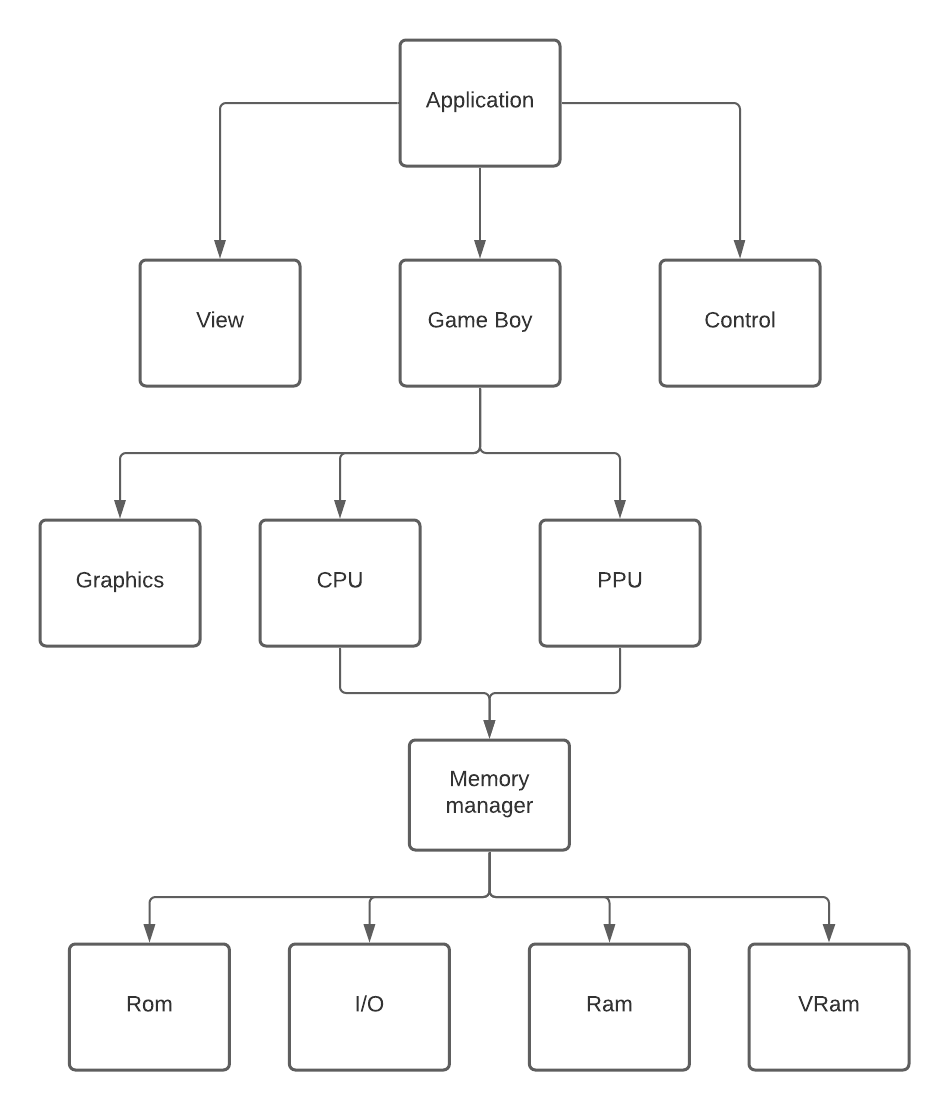
\includegraphics[scale=0.7]{figures/Gameboy Domain model.png}
    \caption{Initial sketch of how different features were to be separated into different modules.}
    \label{fig:initial_domain_model}
\end{figure}

\section{Testing}
Unit tests were one of the methods chosen to ensure that the emulator behaves as intended. For this, Google's testing framework Google Test was used \cite{gtest}. Google Test was chosen as it supports unit tests for C++ and works well with the Continuous Integration (CI) tool Travis \cite{Travis}.
\\\\
%In addition to the use of unit testing, the Game Boy emulator community has developed several test ROMs with the purpose of being able to ensure that the most critical parts of an emulator are behaving correctly \cite{Blargg}. 
Nintendo have not released any official documentation of the hardware and the exact behaviour of the Game Boy is therefore partly unknown. Due to this, one can not be sure of the accuracy of an emulator, and if certain behaviour is correct or not without comparing the emulator to actual hardware. This of course makes development for the Game Boy more difficult. Fortunately, the Game Boy Wiki provides a table for a set of test ROMs \cite{TestROMsResult} made by the emulator community member Blargg \cite{Blargg}, containing the results of running the ROMs on a number of emulators as well as actual hardware. By comparing these results and the results produced when run on a specific emulator, one can in some ways confirm whether or not the emulator is behaving correctly. As the community provides a table with the results from Blargg's test ROMs on actual hardware, these were chosen as the first and main test ROMs to be used. In addition to this, some of the tests were deemed more central than others. Specifically the ROMs testing the instruction timing and instruction behaviour.
%In addition to the use of unit testing, the Game Boy emulator community has developed several test ROMs with the purpose of being able to ensure that the most critical parts of the emulator are behaving correctly \cite{Blargg}. Nintendo has not released any official documentation of the hardware and the exact behaviour of the Game Boy is therefore partly unknown. Due to this, one can not be sure of the accuracy of an emulator, and if certain behaviour is correct or not without comparing the emulator to actual hardware. This of course makes development for the Game Boy more difficult.
%\\\\
%The Game Boy Wiki provides a table for a set of test ROMs made by the emulator community member Blargg \cite{Blargg} \cite{TestROMsResult}, containing the results of running the ROMs on a number of emulators as well as actual hardware.
%By comparing these results and the results produced when ran on a specific emulator, one can in some ways confirm whether or not the emulator is behaving correctly. As the community provides a table with the results from Blargg's test ROMs on actual hardware, these were chosen as the first and main test ROMs to be used. In addition to this, some of the tests were deemed more central than others. Specifically the ROMs testing the instruction timing and instruction behaviour.
\\\\
To streamline the testing process, most of the time spent in unit testing was done testing the basic operations executed by the CPU, MMU, PPU and in time, the APU. This was done to make sure that the most central parts of the emulator work correctly individually. Once this was done, the test ROMs came into use as these require a working CPU, MMU and PPU as they write the results of the tests directly onto the screen. These produce more extensive results and one might argue that they act as integration tests, testing multiple parts of the code and their interactions. In addition to this, testing was also done by playing a multitude of games, visually looking for bugs and otherwise strange behaviour.
%To be able to test the code, the group chose to use 'Google Testing Framework'. GTF  In addition to unit tests the group decided to use specific test ROMs, to test whether specific instructions and interactions between components are implemented correctly.
%Blargg
%Gtest - Unit testing
%Also playable roms in some way, non proprietary. Compare our emulator vs real game-boy regarding these tests: https://gbdev.gg8.se/wiki/articles/Test_ROMs